% -*- coding: utf-8 -*-
%-------------------------designed by zcf--------------
\documentclass[UTF8,a4paper,10pt]{ctexart}
\usepackage[left=3.17cm, right=3.17cm, top=2.74cm, bottom=2.74cm]{geometry}
\usepackage{amsmath}
\usepackage{graphicx,subfig}
\usepackage{float}
\usepackage{cite}
\usepackage{caption}
\usepackage{enumerate}
\usepackage{booktabs} %表格
\usepackage{multirow}
\newcommand{\tabincell}[2]{\begin{tabular}{@{}#1@{}}#2\end{tabular}}  %表格强制换行
%-------------------------字体设置--------------
\usepackage{times} 
\newcommand{\yihao}{\fontsize{26pt}{36pt}\selectfont}           % 一号, 1.4 倍行距
\newcommand{\erhao}{\fontsize{22pt}{28pt}\selectfont}          % 二号, 1.25倍行距
\newcommand{\xiaoer}{\fontsize{18pt}{18pt}\selectfont}          % 小二, 单倍行距
\newcommand{\sanhao}{\fontsize{16pt}{24pt}\selectfont}  %三号字
\newcommand{\xiaosan}{\fontsize{15pt}{22pt}\selectfont}        % 小三, 1.5倍行距
\newcommand{\sihao}{\fontsize{14pt}{21pt}\selectfont}            % 四号, 1.5 倍行距
\newcommand{\banxiaosi}{\fontsize{13pt}{19.5pt}\selectfont}    % 半小四, 1.5倍行距
\newcommand{\xiaosi}{\fontsize{12pt}{18pt}\selectfont}            % 小四, 1.5倍行距
\newcommand{\dawuhao}{\fontsize{11pt}{11pt}\selectfont}       % 大五号, 单倍行距
\newcommand{\wuhao}{\fontsize{10.5pt}{15.75pt}\selectfont}    % 五号, 单倍行距
%-------------------------章节名----------------
\usepackage{ctexcap} 
\CTEXsetup[name={,、},number={ \chinese{section}}]{section}
\CTEXsetup[name={(,)},number={\chinese{subsection}}]{subsection}
\CTEXsetup[name={,.},number={\arabic{subsubsection}}]{subsubsection}
%-------------------------页眉页脚--------------
\usepackage{fancyhdr}
\pagestyle{fancy}
\lhead{\kaishu \leftmark}
% \chead{}
\rhead{\kaishu 计算机系统设计实验报告}%加粗\bfseries 
\lfoot{}
\cfoot{\thepage}
\rfoot{}
\renewcommand{\headrulewidth}{0.1pt}  
\renewcommand{\footrulewidth}{0pt}%去掉横线
\newcommand{\HRule}{\rule{\linewidth}{0.5mm}}%标题横线
\newcommand{\HRulegrossa}{\rule{\linewidth}{1.2mm}}
%-----------------------伪代码------------------
\usepackage{algorithm}  
\usepackage{algorithmicx}  
\usepackage{algpseudocode}  
\floatname{algorithm}{Algorithm}  
\renewcommand{\algorithmicrequire}{\textbf{Input:}}  
\renewcommand{\algorithmicensure}{\textbf{Output:}} 
\usepackage{lipsum}  
\makeatletter
\newenvironment{breakablealgorithm}
  {% \begin{breakablealgorithm}
  \begin{center}
     \refstepcounter{algorithm}% New algorithm
     \hrule height.8pt depth0pt \kern2pt% \@fs@pre for \@fs@ruled
     \renewcommand{\caption}[2][\relax]{% Make a new \caption
      {\raggedright\textbf{\ALG@name~\thealgorithm} ##2\par}%
      \ifx\relax##1\relax % #1 is \relax
         \addcontentsline{loa}{algorithm}{\protect\numberline{\thealgorithm}##2}%
      \else % #1 is not \relax
         \addcontentsline{loa}{algorithm}{\protect\numberline{\thealgorithm}##1}%
      \fi
      \kern2pt\hrule\kern2pt
     }
  }{% \end{breakablealgorithm}
     \kern2pt\hrule\relax% \@fs@post for \@fs@ruled
  \end{center}
  }
\makeatother
%------------------------代码-------------------
\usepackage{xcolor} 
\usepackage{listings} 
\usepackage{fontspec}
\newfontfamily\menlo{Menlo}
\setmonofont[Mapping={}]{Monaco} 
\definecolor{mygreen}{rgb}{0,0.6,0}
\definecolor{mygray}{rgb}{0.5,0.5,0.5}
\definecolor{mymauve}{rgb}{0.58,0,0.82}
\lstset{ %
backgroundcolor=\color{white},   % choose the background color
basicstyle=\footnotesize\ttfamily,        % size of fonts used for the code
columns=fullflexible,
breaklines=true,                 % automatic line breaking only at whitespace
captionpos=b,                    % sets the caption-position to bottom
tabsize=4,
commentstyle=\color{mygreen},    % comment style
escapeinside={\%*}{*)},          % if you want to add LaTeX within your code
keywordstyle=\color{blue},       % keyword style
stringstyle=\color{mymauve}\ttfamily,     % string literal style
frame=single,
rulesepcolor=\color{red!20!green!20!blue!20},
numbers=left,
 numberstyle=\tiny\menlo
% identifierstyle=\color{red},
% language=c++,
}
%------------超链接----------
\usepackage[colorlinks,linkcolor=black,anchorcolor=blue]{hyperref}
%------------------------TODO-------------------
\usepackage{enumitem,amssymb}
\newlist{todolist}{itemize}{2}
\setlist[todolist]{label=$\square$}
% for check symbol 
\usepackage{pifont}
\newcommand{\cmark}{\ding{51}}%
\newcommand{\xmark}{\ding{55}}%
\newcommand{\done}{\rlap{$\square$}{\raisebox{2pt}{\large\hspace{1pt}\cmark}}\hspace{-2.5pt}}
\newcommand{\wontfix}{\rlap{$\square$}{\large\hspace{1pt}\xmark}}
%------------------------水印-------------------
\usepackage{tikz}
\usepackage{xcolor}
\usepackage{eso-pic}

\newcommand{\watermark}[3]{\AddToShipoutPictureBG{
\parbox[b][\paperheight]{\paperwidth}{
\vfill%
\centering%
\tikz[remember picture, overlay]%
  \node [rotate = #1, scale = #2] at (current page.center)%
    {\textcolor{gray!80!cyan!30!magenta!30}{#3}};
\vfill}}}



%———————————————————————————————————————————正文———————————————————————————————————————————————
%----------------------------------------------
\begin{document}
\begin{titlepage}
    \begin{center}
    
\includegraphics[width=0.8\textwidth]{NKU.png}\\[1cm]    
    \textsc{\Huge \kaishu{\textbf{南\ \ \ \ \ \ 开\ \ \ \ \ \ 大\ \ \ \ \ \ 学}} }\\[0.9cm]
    \textsc{\huge \kaishu{\textbf{计\ \ 算\ \ 机\ \ 学\ \ 院}}}\\[0.5cm]
    \textsc{\Large \textbf{计算机系统设计实验报告}}\\[0.8cm]
    \HRule \\[0.9cm]
    { \LARGE \bfseries PA3实验报告}\\[0.4cm]
    \HRule \\[2.0cm]
    \centering
    \textsc{\LARGE \kaishu{朱浩泽\ 1911530}}\\[0.5cm]
    \textsc{\LARGE \kaishu{年级\ :\ 2019级}}\\[0.5cm]
    \textsc{\LARGE \kaishu{专业\ :\ 计算机科学与技术}}\\[0.5cm]
    \textsc{\LARGE \kaishu{指导教师\ :\ 卢冶}}\\[0.5cm]
    \vfill
    {\Large \today}
    \end{center}
\end{titlepage}
% -------------摘------要--------------
\newpage
% \thispagestyle{empty}
% \renewcommand{\abstractname}{\kaishu \sihao \textbf{摘要}}
%     \begin{abstract}

%         \noindent  %顶格
%         \textbf{\\\ 关键字:Parallel}\textbf{} \\\ \\\
%     \end{abstract}
% ----------------------------------------------------------------
\tableofcontents
% ----------------------------------------------------------------
\newpage
\watermark{60}{10}{NKU}
\setcounter{page}{1}
\section{概述}
\subsection{实验目的}
\begin{enumerate}
  \item 了解基础设施测试、调试的基本框架与思想
  \item 实现I/O设备的基本操作
  \item 掌握高级语言程序中的各种类型变量对应的表示形式
  \item 学习指令周期与指令执行过程,并简单实现现代指令系统
  \item 了解冯诺依曼计算机体系结构
  \item 在高级语言程序中的变量、机器数和底层硬件(寄存器、加法器、ALU等)之间建立关联
\end{enumerate}

\subsection{实验内容}
\begin{enumerate}
  \item 实现基本的指令
  \item 运行第一个 C 程序
  \item 补全更多的指令并进行diff-text
  \begin{enumerate}
    \item 完善nemu/src/cpu/exec/exec.c中的opcode\_table
    \item 完善nemu/include/cpu/rtl.h中的基本操作函数
    \item 完善nemu/src/cpu/* 中的执行函数。(执行函数统一通过宏make\_EHelper 定义)
  \end{enumerate}
  \item 学习I/O的原理,实现屏幕的打印和键盘的输入
\end{enumerate}

\section{阶段一}
\subsection{环境配置}
首先,我们要配置好环境变量,由于我在虚拟机终端中使用的是zsh(为了使用oh-my-zsh),所以我们要在zsh的配置中(Home/Username/.zshrc)添加如下内容:
\begin{lstlisting}[]
export NEMU_HOME=~/PA/ics2017/nemu
export AM_HOME=~/PA/ics2017/nexus-am
export NAVY_HOME=~/PA/ics2017/navy-apps
\end{lstlisting}



\subsection{寄存器传输语言}
在程序执行执行过程中,我们都是使用RTL(寄存器传输语言)来实现该过程。首先,需要在 nemu/include/cpu/reg.h 文件中补充EFlags的标志位
\begin{lstlisting}[language=C]
  struct bs {
    unsigned int CF:1;

    unsigned int one:1;
    unsigned int :4;
    unsigned int ZF:1;
    unsigned int SF:1;

    unsigned int :1;
    unsigned int IF:1;
    unsigned int :1;
    unsigned int OF:1;
    unsigned int :20;
  } eflags;
\end{lstlisting}

这些Eflags将在nemu/src/monitor/monitor.c中进行初始化, 并在nemu/src/cpu/arith.c中进行标志位的设置进行减法计算
\begin{lstlisting}[language = C]
static inline void restart() {
  /* Set the initial instruction pointer. */
  cpu.eip = ENTRY_START;

  unsigned int origin = 2;
  memcpy(&cpu.eflags, &origin, sizeof(cpu.eflags));

#ifdef DIFF_TEST
  init_qemu_reg();
#endif
}
\end{lstlisting}
\begin{lstlisting}[language = C]
static inline void eflags_modify() {
  rtl_sub(&t2, &id_dest -> val, &id_src -> val);
  rtl_update_ZFSF(&t2, id_dest -> width);
  rtl_sltu(&t0, &id_dest -> val, &id_src -> val);
  rtl_set_CF(&t0);
  rtl_xor(&t0, &id_dest->val, &id_src->val);
  rtl_xor(&t1, &id_dest->val, &t2);
  rtl_and(&t0, &t0, &t1);
  rtl_msb(&t0, &t0, id_dest->width);
  rtl_set_OF(&t0);
}
\end{lstlisting}

rtl指令在nemu/include/cpu/rtl.h文件中。在rtl.h中,指令分为两部分,一部分是rtl指令,另一部分则是rtl伪指令, 它们是通过rtl指令实现的。

我们实现rtl\_push函数让其修改栈顶,并将指针src1中的内容写入栈。
\begin{lstlisting}[language = C++]
static inline void rtl_push(const rtlreg_t* src1) {
  // esp <- esp - 4
  // M[esp] <- src1
  //TODO();
  rtl_subi(&cpu.esp, &cpu.esp, 4);
  rtl_sm(&cpu.esp, 4, src1);
}
\end{lstlisting}

我们实现rtl\_pop函数让其将rtl\_pop读取的数据写入到通用寄存器中。
\begin{lstlisting}[language = C++]
static inline void rtl_pop(rtlreg_t* dest) {
    // dest <- M[esp]
    rtl_lm(dest,&cpu.esp,4);
    // esp <- esp + 4
    rtl_addi(&cpu.esp,&cpu.esp,4);
  }
\end{lstlisting}

 与此同时,我们还实现了其他指令的编写,如下:

EFLAGS 寄存器的标志位读写函数
\begin{lstlisting}[language = C]
#define make_rtl_arith_logic(name) \
static inline void concat(rtl_, name) (rtlreg_t* dest, const rtlreg_t* src1, const rtlreg_t* src2) { \
  *dest = concat(c_, name) (*src1, *src2); \
} \
static inline void concat3(rtl_, name, i) (rtlreg_t* dest, const rtlreg_t* src1, int imm) { \
  *dest = concat(c_, name) (*src1, imm); \
}
\end{lstlisting}

EFLAGS 寄存器的标志位更新函数
\begin{lstlisting}[language = C]
static inline void rtl_eq0(rtlreg_t* dest, const rtlreg_t* src1) {
  rtl_sltui(dest, src1, 1);
}

static inline void rtl_eqi(rtlreg_t* dest, const rtlreg_t* src1, int imm) {
  rtl_xori(dest, src1, imm);
  rtl_eq0(dest, dest);
}

static inline void rtl_neq0(rtlreg_t* dest, const rtlreg_t* src1) {
  rtl_eq0(dest, src1);
  rtl_eq0(dest, dest);
}

static inline void rtl_msb(rtlreg_t* dest, const rtlreg_t* src1, int width) {
  rtl_shri(dest, src1, width*8-1);
  rtl_andi(dest, dest, 0x1);
}

static inline void rtl_update_ZF(const rtlreg_t* result, int width) {
  rtl_andi(&t0, result, (0xffffffffu >> (4-width)*8));
  rtl_eq0(&t0, &t0);
  rtl_set_ZF(&t0);
}

static inline void rtl_update_SF(const rtlreg_t* result, int width) {
  assert(result != &t0);
  rtl_msb(&t0, result, width);
  rtl_set_SF(&t0);
}
\end{lstlisting}

实现立即数加法
\begin{lstlisting}[language = C]
static inline void rtl_mv(rtlreg_t* dest, const rtlreg_t *src1) {
  rtl_addi(dest, src1, 0);
}
\end{lstlisting}

实现逻辑非运算
\begin{lstlisting}[language = C]
static inline void rtl_not(rtlreg_t* dest) {
  rtl_xori(dest, dest, 0xffffffff);
}
\end{lstlisting}

符号拓展,主要与最高位有关
\begin{lstlisting}[language = C]
static inline void rtl_sext(rtlreg_t* dest, const rtlreg_t* src1, int width) {
  if(width == 0) {
    rtl_mv(dest, src1);
  }
  else {
    rtl_shli(dest, src1, (4 - width) * 8);
    rtl_sari(dest, dest, (4 - width) * 8);
  }
}
\end{lstlisting}

\subsection{尝试运行dummy.c}
首先我们什么都不做,运行 make ARCH=x86-nemu ALL=dummy,一定是报错。我们通过查看反汇编的代码,可以看出是call指令和endbr指令没有实现。我们通过这种方法进行逐一操作,对指令进行补充。
\begin{center}
  \includegraphics*[scale = 0.3]{1.png}
\end{center}

在这一阶段,我们需要实现的指令有如下
\begin{table}[!htbp]
  \centering
  \begin{tabular}{ccccccccccc}
  \toprule  
  指令& 编码\\
  \midrule
  call& e8\\
  push& 50\\
  sub&  83\\
  \bottomrule
  \end{tabular}
  \begin{tabular}{ccccccccccc}
    \toprule  
    指令& 编码\\
    \midrule
    xor& 31\\
    pop& 58\\
    ret& c3\\
    \bottomrule
    \end{tabular}
\end{table}

可以看出,每个指令都有自己的编号,这是通过查阅i386的指令手册来得到的,其第一个16进制数的是指令的opcode。
\begin{center}
  \includegraphics*[scale = 0.35]{2.png}
\end{center}

每条指令分别需要执行函数和译码函数,译码函数的主要作用是从opcode的后三位中读取通用寄存器的编号,过程是读取 decoding.opcode 中标志的寄存器, 将寄存器的内容放入 op->val 中。nemu/src/cpu/exec/exec.c中的opcode\_table的每一条记录包括译码函数、执行函数、(两个)操作数的宽度,如下
\begin{lstlisting}[language = C]
typedef struct {
  DHelper decode;
  EHelper execute;
  int width;
} opcode_entry;
\end{lstlisting}

我们将在这些指令的编号填写在opcode\_table中,如下
\begin{lstlisting}[language = C]
  /* 0x50 */  IDEX(r,push), IDEX(r,push), IDEX(r,push), IDEX(r,push),
  /* 0x54 */  IDEX(r,push), IDEX(r,push), IDEX(r,push), IDEX(r,push),
  //...
  //call
  /* 0xe8 */  IDEX(J,call), IDEX(J,jmp), EMPTY, IDEXW(J,jmp,1),
  ……
\end{lstlisting}

然后在nemu/src/cpu/exec/all-instr.h补全执行函数,如下(一次性全部展示,后续将不再说明)
\begin{lstlisting}[language = C++]
make_EHelper(mov);

make_EHelper(operand_size);

make_EHelper(inv);
make_EHelper(nemu_trap);
make_EHelper(call);
make_EHelper(call_rm);
make_EHelper(push);
make_EHelper(pop);
make_EHelper(sub);
make_EHelper(xor);
make_EHelper(ret);

make_EHelper(endbr);

make_EHelper(add);
make_EHelper(inc);
make_EHelper(dec);
make_EHelper(cmp);
make_EHelper(neg);
make_EHelper(adc);
make_EHelper(sbb);
make_EHelper(mul);
make_EHelper(imul1);
make_EHelper(imul2);
make_EHelper(imul3);
make_EHelper(div);
make_EHelper(idiv);

make_EHelper(not);
make_EHelper(and);
make_EHelper(or);
make_EHelper(xor);
make_EHelper(sal);
make_EHelper(shl);
make_EHelper(shr);
make_EHelper(sar);
make_EHelper(rol);
make_EHelper(setcc);
make_EHelper(test);

make_EHelper(leave);
make_EHelper(cltd);
make_EHelper(cwtl);
make_EHelper(movsx);
make_EHelper(movzx);

make_EHelper(jmp);
make_EHelper(jmp_rm);
make_EHelper(jcc);

make_EHelper(lea);
make_EHelper(nop);

make_EHelper(in);
make_EHelper(out);

make_EHelper(lidt);
make_EHelper(int);

make_EHelper(pusha);
make_EHelper(popa);
make_EHelper(iret);

make_EHelper(mov_store_cr);
\end{lstlisting}

在补充完函数定义后nemu/src/cpu/exec中的执行函数和nemu/src/cpu/exec/decode.c中的译码函数进行编写
\begin{itemize}
  \item push
  
  调用上一节中所写的rtl\_push执行函数进行写栈,代码如下
  \begin{lstlisting}[language = C]
  make_EHelper(push) {
    //TODO();
    rtl_push(&id_dest -> val);
    print_asm_template1(push); 
  }
  \end{lstlisting}
  \item pop
  
  调用上一节中所写的rtl\_pop执行函数进行读栈,将读取的数据写入到通用寄存器中,代码如下
  \begin{lstlisting}[language = C]
make_EHelper(pop) {
  // TODO();
  rtl_pop(&t2);
  operand_write(id_dest, &t2);
  print_asm_template1(pop);
}
\end{lstlisting}
  
\item call
    
为J形指令,操作数仅一个立即数。CPU 的跳转目标地址=当前 eip+立即数 offset。所以我们编写nemu/src/cpu/decode/decode.c中的译码函数make\_DHelper(J),调用decode\_op\_SI 函数实现立即数的读取,并更新jmp\_eip。
\begin{lstlisting}[language = C]
make_DHelper(J) {
  decode_op_SI(eip, id_dest, false);
  // the target address can be computed in the decode stage
  decoding.jmp_eip = id_dest->simm + *eip;
}  
\end{lstlisting}
然后我们编写nemu/src/cpu/exe/control.c中的执行函数make\_EHelper(call)
\begin{lstlisting}[language = C]
make_EHelper(call) {
  // the target address is calculated at the decode stage
  //TODO();
  rtl_li(&t2, decoding.seq_eip);
  rtl_push(&t2);

  decoding.is_jmp = 1;

  print_asm("call %x", decoding.jmp_eip);
}
\end{lstlisting}
  \item sub
  
  编写译码函数make\_DHelper(I2a),调用 decode\_op\_a读取 AX/EAX中的数据写入 id\_dest,调用 decode\_op\_I 读取立即数并存入 id\_src
  \begin{lstlisting}[language = C]
make_DHelper(I2a) {
  decode_op_a(eip, id_dest, true);
  decode_op_I(eip, id_src, true);
}
\end{lstlisting}
  编写执行函数make\_EHelper(sub),调用 eflags\_modify()计算减法并将值写回寄存器
  \begin{lstlisting}[language = C]
make_EHelper(sub) {
  // TODO();

  eflags_modify();
  operand_write(id_dest, &t2);
  print_asm_template2(sub);
}
\end{lstlisting}

  \item xor
  
  实现执行函数make\_Ehelper(xor)
  \begin{lstlisting}[language = C]
make_EHelper(xor) {
  // TODO();
  rtl_xor(&t2, &id_dest -> val, &id_src -> val);
  operand_write(id_dest, &t2);

  rtl_update_ZFSF(&t2, id_dest -> width);

  rtl_set_CF(&tzero);
  rtl_set_OF(&tzero);

  print_asm_template2(xor);
}
\end{lstlisting}

  \item ret
  
  实现执行函数make\_EHelper(ret),用栈的数据修改IP的内容,实现近转移
  \begin{lstlisting}[language = C]
make_EHelper(ret) {
  // TODO();
  rtl_pop(&t2);
  decoding.jmp_eip = t2;
  decoding.is_jmp = 1;
  print_asm("ret");
}
\end{lstlisting}
\end{itemize}

\subsection{实验结果}
在补充完这些所需要的指令后,我们再次执行 make ARCH=x86-nemu ALL=dummy,可以看到这时dummy.c可以在我们的nemu中正确的运行。
\begin{center}
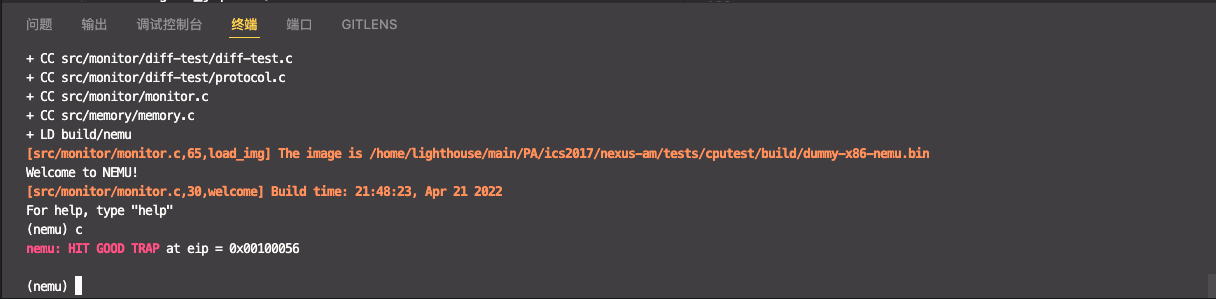
\includegraphics[width=0.9\textwidth]{dummy.png}
\end{center}


我们可以看出,指令执行的大概过程是在exec.c中,我们通过exec\_wrapper()函数开始执行指令,将当前的eip放进译码信息中(主要是为了诸如jmp,call等转移指令),之后执行exec\_real()函数。在该函数中,我们首先从当前地址中取出一个字节。在指令集执行过程中,我们都是先取 出一个字节的操作码,从opcode\_table中寻找匹配项,再执行对应的译码程序和执行程序,完成程序指令的执行。具体来说,就是将当前的 \%eip 保存到全局译码信息 decoding 的成员 seq\_eip 中,然后将其地址被作为参数 送进 exec\_real() 函数。当代码从 exec\_real() 返回时, decoding.seq\_eip 将会指向下一条指令的地址,调用 idex() 对指令进行进一步的译码和执行。

\section{阶段二}
在阶段二中,需要我们进一步补全代码,并进行对应的diff-test对代码正确性进
行检验
\subsection{代码补全}
\begin{itemize}
  \item mov
  \begin{lstlisting}[language = C++]
make_EHelper(mov) {
  operand_write(id_dest, &id_src->val);
  print_asm_template2(mov);
}
  \end{lstlisting}
  \item leave
  \begin{lstlisting}[language = C]
make_EHelper(leave) {
  // TODO();

  rtl_mv(&cpu.esp, &cpu.ebp);
  rtl_pop(&cpu.ebp);
  print_asm("leave");
}
\end{lstlisting}
  \item and
  \begin{lstlisting}[language = C]
make_EHelper(and) {
  // TODO();
  
  rtl_and(&t2,&id_dest->val,&id_src->val);
  operand_write(id_dest,&t2);
  rtl_update_ZFSF(&t2,id_dest->width);
  rtl_set_CF(&tzero);
  rtl_set_OF(&tzero);
  print_asm_template2(and);
}
\end{lstlisting}
  
  在i386手册中为CBW和CWD,CBW为在EAX内字节到字的转换,和字到双字的 转换,CWD为在EAX和EDX间的转换

  \item movsx/movzx
  
  因为id\_src和id\_dest两者的宽度并不相同,所以在进入函数 时会重新调整id\_dest的宽度,这意味我们填写译码函数时,按照id\_src的宽度去填 写就可以了。(我们是在执行函数中才更正了id\_dest的宽度,print出的结果没有随之更正,但不影响程序执行的结果)
  \begin{lstlisting}[language = C]
make_EHelper(movsx) {
  id_dest->width = decoding.is_operand_size_16 ? 2 : 4;
  rtl_sext(&t2, &id_src->val, id_src->width);
  operand_write(id_dest, &t2);
  print_asm_template2(movsx);
}
    
make_EHelper(movzx) {
  id_dest->width = decoding.is_operand_size_16 ? 2 : 4;
  operand_write(id_dest, &id_src->val);
  print_asm_template2(movzx);
}
\end{lstlisting}
\item add

add同sub,需要修改的地方主要是CF和OF的判别
\begin{lstlisting}[language = C]
  make_EHelper(add) {
  // TODO();

  rtl_add(&t2, &id_dest->val, &id_src->val);
  operand_write(id_dest, &t2);

  rtl_update_ZFSF(&t2, id_dest->width);

  rtl_sltu(&t0, &t2, &id_dest->val);
  rtl_set_CF(&t0);

  rtl_xor(&t0, &id_src->val, &t2);
  rtl_xor(&t1, &id_dest->val, &t2);
  rtl_and(&t0, &t0, &t1);
  rtl_msb(&t0, &t0, id_dest->width);
  rtl_set_OF(&t0);
  print_asm_template2(add);
}
\end{lstlisting}
\item inc 
\begin{lstlisting}[language = C]
  make_EHelper(inc) {
  //TODO();

  rtl_addi(&t2, &id_dest->val, 1);
  operand_write(id_dest, &t2);
  rtl_update_ZFSF(&t2, id_dest->width);
  rtl_eqi(&t0, &t2, 0x80000000);
  rtl_set_OF(&t0);
  print_asm_template1(inc);
}
\end{lstlisting}
\item dec
\begin{lstlisting}[language = C]
  make_EHelper(dec) {
  // TODO();

  rtl_subi(&t2, &id_dest->val, 1);
  operand_write(id_dest, &t2);
  rtl_update_ZFSF(&t2, id_dest->width);
  rtl_eqi(&t0, &t2, 0x7fffffff);
  rtl_set_OF(&t0);
  print_asm_template1(dec);
}
\end{lstlisting}
\item cmp
\begin{lstlisting}[language = C]
  make_EHelper(cmp) {
  // TODO();

  eflags_modify();

  print_asm_template2(cmp);
}
\end{lstlisting}
\item neg

二进制补码取反
\begin{lstlisting}[language = C]
make_EHelper(neg) {
  // TODO();

  rtl_sub(&t2, &tzero, &id_dest->val);
  rtl_update_ZFSF(&t2, id_dest->width);
  rtl_neq0(&t0,&id_dest->val);
  rtl_set_CF(&t0);
  rtl_eqi(&t0,&id_dest->val,0x80000000);
  rtl_set_OF(&t0);
  operand_write(id_dest,&t2);
  print_asm_template1(neg);
}
\end{lstlisting}
\item or 
\begin{lstlisting}[language = C]
make_EHelper(or) {
  // TODO();

  rtl_or(&t2,&id_dest->val,&id_src->val);
  operand_write(id_dest,&t2);
  rtl_update_ZFSF(&t2,id_dest->width);
  rtl_set_CF(&tzero);
  rtl_set_OF(&tzero);
  print_asm_template2(or);

  print_asm_template2(or);
}
\end{lstlisting}
\item not 
\begin{lstlisting}[language = C]
make_EHelper(not) {
  // TODO();

  rtl_not(&id_dest->val);
  operand_write(id_dest,&id_dest->val);
  print_asm_template1(not);
}
\end{lstlisting}
\item cltd 

当于 cdq 指令,作用是把 eax 的 32 位整数扩展 为 64 位,高 32 位用 eax 的符号位填充保存到edx,或 ax 的 16 位整数扩展为 32 位,高 16 位用 ax 的符号位填充保存到 dx
\begin{lstlisting}[language = C]
make_EHelper(cltd) {
  if (decoding.is_operand_size_16) {
    // TODO();
    rtl_lr_w(&t0, R_AX);
    rtl_sext(&t0, &t0, 2);
    rtl_sari(&t0, &t0, 31);
    rtl_sr_w(R_DX, &t0);
  }
  else {
    // TODO();
    rtl_sari(&cpu.edx, &cpu.eax, 31);
  }

  print_asm(decoding.is_operand_size_16 ? "cwtl" : "cltd");
}
\end{lstlisting}
\item leave

将栈指针指向帧指针,然后 pop 备份的原帧指针到\%ebp
\begin{lstlisting}[language = C]
make_EHelper(leave) {
  // TODO();

  rtl_mv(&cpu.esp, &cpu.ebp);
  rtl_pop(&cpu.ebp);
  print_asm("leave");
}
\end{lstlisting}
\item 补全的指令表
\begin{lstlisting}[language = C]
  /* 0x80, 0x81, 0x83 */
make_group(gp1,
    EX(add), EX(or), EX(adc), EX(sbb),
    EX(and), EX(sub), EX(xor), EX(cmp))

  /* 0xc0, 0xc1, 0xd0, 0xd1, 0xd2, 0xd3 */
make_group(gp2,
    EX(rol), EMPTY, EMPTY, EMPTY,
    EX(shl), EX(shr), EMPTY, EX(sar))

  /* 0xf6, 0xf7 */
make_group(gp3,
    IDEX(test_I, test), EMPTY, EX(not), EX(neg),
    EX(mul), EX(imul1), EX(div), EX(idiv))

  /* 0xfe */
make_group(gp4,
    EX(inc), EX(dec), EMPTY, EMPTY,
    EMPTY, EMPTY, EMPTY, EMPTY)

  /* 0xff */
make_group(gp5,
    EX(inc), EX(dec), EX(call_rm), EMPTY,
    EX(jmp_rm), EMPTY, EX(push), EMPTY)

  /* 0x0f 0x01*/
make_group(gp7,
    EMPTY, EMPTY, EMPTY, EMPTY,
    EMPTY, EMPTY, EMPTY, EMPTY)

/* TODO: Add more instructions!!! */

opcode_entry opcode_table [512] = {
  /* 0x00 */	IDEXW(G2E, add, 1), IDEX(G2E, add), IDEXW(E2G, add, 1), IDEX(E2G, add),
  /* 0x04 */	IDEXW(I2a, add, 1), IDEX(I2a, add), EMPTY, EMPTY,
  /* 0x08 */	IDEXW(G2E, or, 1), IDEX(G2E, or), IDEXW(E2G, or, 1), IDEX(E2G, or),
  /* 0x0c */	IDEXW(I2a, or, 1), IDEX(I2a, or), EMPTY, EX(2byte_esc),
  /* 0x10 */	IDEXW(G2E, adc, 1), IDEX(G2E, adc), IDEXW(E2G, adc, 1), IDEX(E2G, adc),
  /* 0x14 */	IDEXW(I2a, adc, 1), IDEX(I2a, adc), EMPTY, EMPTY,
  /* 0x18 */	IDEXW(G2E, sbb, 1), IDEX(G2E, sbb), IDEXW(E2G, sbb, 1), IDEX(E2G, sbb),
  /* 0x1c */	IDEXW(I2a, sbb, 1), IDEX(I2a, sbb), EMPTY, EMPTY,
  /* 0x20 */	IDEXW(G2E, and, 1), IDEX(G2E, and), IDEXW(E2G, and, 1), IDEX(E2G, and),
  /* 0x24 */	IDEXW(I2a, and, 1), IDEX(I2a, and), EMPTY, EMPTY,
  /* 0x28 */	IDEXW(G2E, sub, 1), IDEX(G2E, sub), IDEXW(E2G, sub, 1), IDEX(E2G, sub),
  /* 0x2c */	IDEXW(I2a, sub, 1), IDEX(I2a, sub), EMPTY, EMPTY,
  /* 0x30 */	IDEXW(G2E, xor, 1), IDEX(G2E, xor), IDEXW(E2G, xor, 1), IDEX(E2G, xor),
  /* 0x34 */	IDEXW(I2a, xor, 1), IDEX(I2a, xor), EMPTY, EMPTY,
  /* 0x38 */	IDEXW(G2E, cmp, 1), IDEX(G2E, cmp), IDEXW(E2G, cmp, 1), IDEX(E2G, cmp),
  /* 0x3c */	IDEXW(I2a, cmp, 1), IDEX(I2a, cmp), EMPTY, EMPTY,
  /* 0x40 */	IDEX(r, inc), IDEX(r, inc), IDEX(r, inc), IDEX(r, inc),
  /* 0x44 */	IDEX(r, inc), IDEX(r, inc), IDEX(r, inc), IDEX(r, inc),
  /* 0x48 */	IDEX(r, dec), IDEX(r, dec), IDEX(r, dec), IDEX(r, dec),
  /* 0x4c */	IDEX(r, dec), IDEX(r, dec), IDEX(r, dec), IDEX(r, dec),
  /* 0x50 */	IDEX(r, push), IDEX(r, push), IDEX(r, push), IDEX(r, push),
  /* 0x54 */	IDEX(r, push), IDEX(r, push), IDEX(r, push), IDEX(r, push),
  /* 0x58 */	IDEX(r, pop), IDEX(r, pop), IDEX(r, pop), IDEX(r, pop),
  /* 0x5c */	IDEX(r, pop), IDEX(r, pop), IDEX(r, pop), IDEX(r, pop),
  /* 0x60 */	EMPTY, EMPTY, EMPTY, EMPTY,
  /* 0x64 */	EMPTY, EMPTY, EX(operand_size), EMPTY,
  /* 0x68 */	IDEX(I, push), IDEX(I_E2G, imul3), IDEXW(push_SI, push, 1), IDEX(SI_E2G, imul3),
  /* 0x6c */	EMPTY, EMPTY, EMPTY, EMPTY,
  /* 0x70 */	IDEXW(J, jcc, 1), IDEXW(J, jcc, 1), IDEXW(J, jcc, 1), IDEXW(J, jcc, 1),
  /* 0x74 */	IDEXW(J, jcc, 1), IDEXW(J, jcc, 1), IDEXW(J, jcc, 1), IDEXW(J, jcc, 1),
  /* 0x78 */	IDEXW(J, jcc, 1), IDEXW(J, jcc, 1), IDEXW(J, jcc, 1), IDEXW(J, jcc, 1),
  /* 0x7c */	IDEXW(J, jcc, 1), IDEXW(J, jcc, 1), IDEXW(J, jcc, 1), IDEXW(J, jcc, 1),
  /* 0x80 */	IDEXW(I2E, gp1, 1), IDEX(I2E, gp1), EMPTY, IDEX(SI2E, gp1),
  /* 0x84 */	IDEXW(G2E, test, 1), IDEX(G2E, test), EMPTY, EMPTY,
  /* 0x88 */	IDEXW(mov_G2E, mov, 1), IDEX(mov_G2E, mov), IDEXW(mov_E2G, mov, 1), IDEX(mov_E2G, mov),
  /* 0x8c */	EMPTY, IDEX(lea_M2G, lea), EMPTY, IDEX(E, pop),
  /* 0x90 */	EX(nop), EMPTY, EMPTY, EMPTY,
  /* 0x94 */	EMPTY, EMPTY, EMPTY, EMPTY,
  /* 0x98 */	EMPTY, EX(cltd), EMPTY, EMPTY,
  /* 0x9c */	EMPTY, EMPTY, EMPTY, EMPTY,
  /* 0xa0 */	IDEXW(O2a, mov, 1), IDEX(O2a, mov), IDEXW(a2O, mov, 1), IDEX(a2O, mov),
  /* 0xa4 */	EMPTY, EMPTY, EMPTY, EMPTY,
  /* 0xa8 */	IDEXW(I2a, test, 1), IDEX(I2a, test), EMPTY, EMPTY,
  /* 0xac */	EMPTY, EMPTY, EMPTY, EMPTY,
  /* 0xb0 */	IDEXW(mov_I2r, mov, 1), IDEXW(mov_I2r, mov, 1), IDEXW(mov_I2r, mov, 1), IDEXW(mov_I2r, mov, 1),
  /* 0xb4 */	IDEXW(mov_I2r, mov, 1), IDEXW(mov_I2r, mov, 1), IDEXW(mov_I2r, mov, 1), IDEXW(mov_I2r, mov, 1),
  /* 0xb8 */	IDEX(mov_I2r, mov), IDEX(mov_I2r, mov), IDEX(mov_I2r, mov), IDEX(mov_I2r, mov),
  /* 0xbc */	IDEX(mov_I2r, mov), IDEX(mov_I2r, mov), IDEX(mov_I2r, mov), IDEX(mov_I2r, mov),
  /* 0xc0 */	IDEXW(gp2_Ib2E, gp2, 1), IDEX(gp2_Ib2E, gp2), EMPTY, EX(ret),
  /* 0xc4 */	EMPTY, EMPTY, IDEXW(mov_I2E, mov, 1), IDEX(mov_I2E, mov),
  /* 0xc8 */	EMPTY, EX(leave), EMPTY, EMPTY,
  /* 0xcc */	EMPTY, EMPTY, EMPTY, EMPTY,
  /* 0xd0 */	IDEXW(gp2_1_E, gp2, 1), IDEX(gp2_1_E, gp2), IDEXW(gp2_cl2E, gp2, 1), IDEX(gp2_cl2E, gp2),
  /* 0xd4 */	EMPTY, EMPTY, EX(nemu_trap), EMPTY,
  /* 0xd8 */	EMPTY, EMPTY, EMPTY, EMPTY,
  /* 0xdc */	EMPTY, EMPTY, EMPTY, EMPTY,
  /* 0xe0 */	EMPTY, EMPTY, EMPTY, EMPTY,
  /* 0xe4 */	IDEXW(in_I2a, in, 1), IDEXW(in_I2a, in, 1), IDEXW(out_a2I, out, 1), IDEXW(out_a2I, out, 1),
  /* 0xe8 */	IDEX(J, call), IDEX(J, jmp), EMPTY, IDEXW(J, jmp, 1),
  /* 0xec */	IDEXW(in_dx2a, in, 1), IDEX(in_dx2a, in), IDEXW(out_a2dx, out, 1), IDEX(out_a2dx, out),
  /* 0xf0 */  EMPTY, EMPTY, EMPTY, EXW(endbr, 3),
  /* 0xf4 */	EMPTY, EMPTY, IDEXW(E, gp3, 1), IDEX(E, gp3),
  /* 0xf8 */	EMPTY, EMPTY, EMPTY, EMPTY,
  /* 0xfc */	EMPTY, EMPTY, IDEXW(E, gp4, 1), IDEX(E, gp5),

  /*2 byte_opcode_table */

  /* 0x00 */	EMPTY, IDEX(gp7_E, gp7), EMPTY, EMPTY,

  ……

  /* 0x80 */	IDEX(J, jcc), IDEX(J, jcc), IDEX(J, jcc), IDEX(J, jcc),
  /* 0x84 */	IDEX(J, jcc), IDEX(J, jcc), IDEX(J, jcc), IDEX(J, jcc),
  /* 0x88 */	IDEX(J, jcc), IDEX(J, jcc), IDEX(J, jcc), IDEX(J, jcc),
  /* 0x8c */	IDEX(J, jcc), IDEX(J, jcc), IDEX(J, jcc), IDEX(J, jcc),
  /* 0x90 */	IDEXW(E, setcc, 1), IDEXW(E, setcc, 1), IDEXW(E, setcc, 1), IDEXW(E, setcc, 1),
  /* 0x94 */	IDEXW(E, setcc, 1), IDEXW(E, setcc, 1), IDEXW(E, setcc, 1), IDEXW(E, setcc, 1),
  /* 0x98 */	IDEXW(E, setcc, 1), IDEXW(E, setcc, 1), IDEXW(E, setcc, 1), IDEXW(E, setcc, 1),
  /* 0x9c */	IDEXW(E, setcc, 1), IDEXW(E, setcc, 1), IDEXW(E, setcc, 1), IDEXW(E, setcc, 1),
  /* 0xa0 */	EMPTY, EMPTY, EMPTY, EMPTY,
  /* 0xa4 */	EMPTY, EMPTY, EMPTY, EMPTY,
  /* 0xa8 */	EMPTY, EMPTY, EMPTY, EMPTY,
  /* 0xac */	EMPTY, EMPTY, EMPTY, IDEX(E2G, imul2),
  /* 0xb0 */	EMPTY, EMPTY, EMPTY, EMPTY,
  /* 0xb4 */	EMPTY, EMPTY, IDEXW(mov_E2G, movzx, 1), IDEXW(mov_E2G, movzx, 2),
  /* 0xb8 */	EMPTY, EMPTY, EMPTY, EMPTY,
  /* 0xbc */	EMPTY, EMPTY, IDEXW(mov_E2G, movsx, 1), IDEXW(mov_E2G, movsx, 2),
};
\end{lstlisting}
\item 补全nemu/src/cpu/exec/cc.c中的rtl\_setcc函数
\begin{lstlisting}[language = C]
  switch (subcode & 0xe) {
    case CC_O:
	    rtl_get_OF(dest);
	    break;	
    case CC_B:
	    rtl_get_CF(dest);
	    break;
    case CC_E:
	    rtl_get_ZF(dest);
	    break;
    case CC_BE:
	    assert(dest!=&t0);
	    rtl_get_CF(dest);
	    rtl_get_ZF(&t0);
      rtl_or(dest,dest,&t0);
      break;
    case CC_S:
	    rtl_get_SF(dest);
	    break;
    case CC_L:
	    assert(dest!=&t0);
	    rtl_get_SF(dest);
	    rtl_get_OF(&t0);
      rtl_xor(dest,dest,&t0);
	    break;
    case CC_LE:
	    assert(dest!=&t0);
	    rtl_get_SF(dest);
	    rtl_get_OF(&t0);
      rtl_xor(dest,dest,&t0);
	    rtl_get_ZF(&t0);
	    rtl_or(dest,dest,&t0);
	    break;
    default: 
      panic("should not reach here");
    case CC_P: 
      panic("n86 does not have PF");
  }
\end{lstlisting}
\item 此外,需要补充nemu/src/cpu/decode.c中的make\_DopHelper(SI)函数
\begin{lstlisting}[language = C]
static inline make_DopHelper(I) {
  /* eip here is pointing to the immediate */
  op->type = OP_TYPE_IMM;
  op->imm = instr_fetch(eip, op->width);
  rtl_li(&op->val, op->imm);

#ifdef DEBUG
  snprintf(op->str, OP_STR_SIZE, "$0x%x", op->imm);
#endif
}
\end{lstlisting}

\end{itemize}
\subsection{Differential Testing}
每执行一条指令之后,为了及时地捕捉到 error,让 NEMU 和 QEMU 逐条指令地执行同一个客户程序,都会检查各自的寄存器和内存的状态,根据手册,这里不需要比 较eflags是否相同,因为有一些指令我们实现的并不一样。

\begin{lstlisting}[language = C]
  if(r.eax!=cpu.eax) {
    diff=true;
  }
  if(r.ecx!=cpu.ecx) {
    diff=true;
  }
  if(r.edx!=cpu.edx) {
    diff=true;
  }
  if(r.ebx!=cpu.ebx) {
    diff=true;
  }
  if(r.esp!=cpu.esp) {
	  diff=true;
  }
  if(r.ebp!=cpu.ebp) {
	  diff=true;
  }
  if(r.esi!=cpu.esi) {
	  diff=true;
  }
  if(r.edi!=cpu.edi) {
	  diff=true;
  }
  if (diff) {
    nemu_state = NEMU_END;
  }
  if(r.eip!=cpu.eip) {
	  diff=true;
	  Log("different:qemu.eip=0x%x,nemu.eip=0x%x",r.eip,cpu.eip);
  }
\end{lstlisting}
\subsection{实验结果}
\begin{center}
  \includegraphics*[scale = 0.25]{runall}
\end{center}
\section{阶段三}
在nemu中,提供了端口映射和内存映射,后者主要用于显示画面,在
nemu/include/common.h中定义宏HAS\_IOE后,即可加入IOE。
\subsection{串口}
in 指令用于将设备寄存器中的数据传输到 CPU 寄存器中,out指令用于将 CPU 寄存器中的数据传送到设备寄存器中。
\begin{lstlisting}[language = C]
make_EHelper(in) {
  // TODO();
  rtl_li(&t0, pio_read(id_src -> val, id_dest -> width));
  operand_write(id_dest, &t0);
  print_asm_template2(in);

#ifdef DIFF_TEST
  diff_test_skip_qemu();
#endif
}

make_EHelper(out) {
  // TODO();
  pio_write(id_dest -> val, id_src -> width, id_src -> val);

  print_asm_template2(out);

#ifdef DIFF_TEST
  diff_test_skip_qemu();
#endif
}
\end{lstlisting}
调用port-io程序中给出的写数据和读数据的端口即可,测试hello world
\begin{center}
  \includegraphics*[scale = 0.25]{hello world.png}
\end{center}

\subsection{时钟}
在nexus-am/am/arch/x86-nemu/src/ioe.c中实现即可,我们看到初始化时, 已经给我们提供了样例,可以一样的方式添加。
\begin{lstlisting}[language = C]
unsigned long _uptime() {
  unsigned long ms = inl(RTC_PORT) - boot_time;
  return ms;
}
\end{lstlisting}
time-test运行
\begin{center}
  \includegraphics*[scale = 0.3]{time.png}
\end{center}
跑分测试,可以看出,这性能是相当的差。
  \begin{center}
    \includegraphics*[scale = 0.3]{paofen1.png}
  \end{center}
  
\subsection{键盘I/O}
键盘也是利用端口映射实现,当有按键按下时,状态寄存器会设置为1,观察 keyboard.c可以发现,他将按下的键存在一个长为1024的数组中,访问时,会先访 问状态寄存器,若队列不为空或者其值为1,则访问数据寄存器获得对应的值。(在这里开始需要使用图形化界面,所以我们不得不配置图形化界面)
\begin{lstlisting}[language = C]
int _read_key() {
  uint32_t key_code = _KEY_NONE;
  if (inb(I8042_STATUS_PORT) )
      key_code = inl(I8042_DATA_PORT);
  return key_code;
}
\end{lstlisting}
\begin{center}
  \includegraphics*[scale = 0.35]{keu}
\end{center}

可以看到可以检测到同时按下多个按键,当发送的数字为键盘码+0x8000 时,意味着键盘被按下,而当单纯发送键盘码时,意味着键盘被抬起,这样来判断按键是否是在一起被按下。

\subsection{VGA}
在 paddr\_read() 和 paddr\_write() 中加入对内存映射 I/O 的判断。通过 is\_mmio() 函数判断一个物 理地址是否被映射到 I/O 空间,如果是, is\_mmio() 会返回映射号,否则返回-1。内存映射 I/O 的访问 需要调用 mmio\_read() 或 mmio\_write() ,调用时需要提供映射号。如果不是内存映射 I/O 的访问, 就访问 pmem。需要在nemu/src/memory/memory.c中引用头文件device/mmio.h,相当于我们将一系列io放入了内存中
\begin{lstlisting}[language = C]
#include "device/mmio.h"

uint32_t paddr_read(paddr_t addr, int len) {
  int r = is_mmio(addr);
  if(r == -1) {
    return pmem_rw(addr, uint32_t) & (~0u >> ((4 - len) << 3));
  }
  else {
    return mmio_read(addr, len, r);
  }
}

void paddr_write(paddr_t addr, int len, uint32_t data) {
  int r = is_mmio(addr);
  if(r == -1){
    memcpy(guest_to_host(addr), &data, len);
  }
  else {
    mmio_write(addr, len, data, r);
  }
}
\end{lstlisting}

在nexus-am/am/arch/x86-nemu/src/ioe.c中实现\_draw\_rect()函数,将一个矩阵中像素赋值,注意赋值的顺序
\begin{lstlisting}[language = C]
void _draw_rect(const uint32_t *pixels, int x, int y, int w, int h) {
  // int i;
  // for (i = 0; i < _screen.width * _screen.height; i++) {
  //   fb[i] = i;
  // }
  int temp = (w > _screen.width - x)?_screen.width -x :w;
  int cp_bytes = sizeof(uint32_t) *temp;
  for(int j = 0; j < h && y + j < _screen.height; j++) {
    memcpy(&fb[(y + j) * _screen.width + x], pixels, cp_bytes);
    pixels += w;
  }
}
\end{lstlisting}
运行结果
\begin{center}
  \includegraphics*[scale = 0.2]{h}
\end{center}
\subsection{运行打字游戏}
\begin{center}
  \includegraphics*[scale = 0.35]{game}
\end{center}

\section{必答题}
\subsection{第一题}
\textbf{在nemu/include/cpu/rtl.h中,你会看到由staticinline开头定义的各种RTL指令函数.选择其中一个函数,分别尝试去掉 static,去掉 inline 或去掉两者,然后重新进行编译,你会看到发生错误。请分别解释为什么会发生这些错误?你有办法证明你的想法吗?}
\begin{enumerate}
  \item 去掉static
  
  首先我们去掉rtl\_push的static进行尝试,结果如下
  \begin{center}
    \includegraphics*[scale = 0.25]{ahh}
  \end{center}
  可以看到,无事发生。去掉static后就变成了内联函数。inline是向编译器建议,将被inline修饰的函数以内联的方式嵌入到调用 这个函数的地方。但这不是强制的,编译器的优化程度和最终是否内联也有关系。而static inline会以一 种类似于宏定义的方式,将调用被static inline修饰的函数的语句替换为那个函数体对应的指令,所以 static inline 是强制内联。所以去掉static后,编译器没有进行强制内联的话,该函数就相当于是一个普通函数。
  \item 去掉inline
  
  然后我们去掉rtl\_push的inline进行尝试
  \begin{center}
    \includegraphics*[scale = 0.25]{pupu}
  \end{center}
  会出现定义但未使用的问题。这是因为去掉inline后函数变成了静态函数,只能在该文件中被引用。而该rtl.h文件中并没有引用rtl\_mv函 数,而是在exe文件夹下的*.c文件中引用了。

  \item inline和static都去掉
  
  我们去掉rtl\_push的inline和static进行尝试。
  \begin{center}
    \includegraphics*[scale = 0.25]{false}
  \end{center}
  出现重复定义的情况。这是因为exe文件夹下的.c文件中都引用了rtl.h文件,编译的时候这些文件和rtl.h 文件中都有了rtl\_mv函数的定义,导致了多次定义。而如果是static inline 或者是static,是将该函数的 使用限定在了该源文件中,允许其它文件中的重复定义,所以不会报错。


\end{enumerate}

\subsection{第二题}
\textbf{了解Makefile请描述你在nemu目录下敲入make后,make程序如何组织.c和.h文件,最终生成可执行文件nemu/build/nemu.(这个问题包括两个方面:Makefile 的工作方式和编译链接的过程.)关于 Makefile 工作 方式的提示:Makefile 中使用了变量,包含文件等特性;Makefile 运用并重写了一些 implicit rules;在 man make 中搜索-n 选项,也许会对你有帮助;RTFM}

makefile的各条指令可以概括为以下具体形式,下一行的content前面一定要有tab, instr用于指定obj文件,src指定依赖文件,content是具体的原 来需要在cmd中输入的指令,有时候为了书写的鲁棒性和可复用性,可以定义一些变量(前面用\$符号 表示)
\begin{lstlisting}[]
dest/instr: src
  content
\end{lstlisting}
当执行make时,make会在当前目录下搜索Makefile,执行相应的操作。make首先会判断原始代码是 否经过变动了,会自动更新执行。
是否更新执行的条件:
如果这个工程没有编译过,那么我们的所有C文件都要编译并被链接。 如果这个工程的某几个C文件被修改,那么我们只编译被修改的C文件,并链接目标程序。 如果这个工程的头文件被改变了,那么我们需要编译引用了这几个头文件的C文件,并链接目标程 序。
所以make在会根据c文件的依赖关系自动推导进行编译,编译出.o文件。然后是链接目标程序。链接 时,主要是链接函数和全局变量以及指令中指定的库文件。


\section{感想与体会}
首先就是在运行dummy时候遇到的第一个bug,出现了一个叫endbr32的指令,这个指令通过查阅i386手册没有获得任何信息
\begin{center}
  \includegraphics*[scale = 0.5]{截屏2022-03-29 00.17.26.png}
  \includegraphics*[scale = 0.5]{截屏2022-03-29 00.17.28.png}
\end{center}
通过上网搜索这个问题,我们可以看到,所有提出这个问题的基本都是在做本实验,甚至有几个还能看出来是上届的一位学长。这个问题通过搜索可以确定是由于本实验应该跑在32位的机器上而我是用的是64位的机器的原因。但是通过网上的解答不太能获得实质性的解决,多半是要更改编译选项来骗过编译器。于是我们索性将这条指令当作正常的指令对待,通过查阅反汇编代码,我们构造这个指令的执行函数于nemu/src/cpu/exec/special.c中
\begin{lstlisting}[language
  =C]]  
make_EHelper(endbr) {
    instr_fetch(eip, id_src -> width);
    print_asm("endbr32");
}
\end{lstlisting}
并在指令表中添加
\begin{lstlisting}[language=C]
  /* 0xf0 */  EMPTY, EMPTY, EMPTY, EXW(endbr, 3),
\end{lstlisting}
然后这个问题得到了顺利的解决,希望可以一劳永逸,但是听说以后还会有架构的问题,我就很害怕。

遇到的第二个问题,就是opcode有一位的和两位的,最开始没有注意,全部填写在了一位的部分,这样导致了指令长度的问题,反映出来的结果就是指令的报错。这个bug找了好久,最后还是粗心的问题。

遇到的第三个问题,就比较严重。因为我是用的是苹果的m1电脑,是arm架构的,安装x86的虚拟机比较麻烦,所以选择了租用腾讯云服务器。在PA1的时候,使用ssh连接,使用体验感不错。可是到了PA2需要进行输入输出流,只有命令行进行操作扁成了一个大问题,可能会导致实验无法完成。于是查阅了资料,通过sudo apt-get install tasksel -y命令成功安装了图形化界面,可是这时候又出现了问题,ssh只能连接到命令行,不能连接图形化界面。尝试使用teamviewer进行连接,结果掉帧严重,简直无法使用。于是通过查阅资料得知可以使用snv进行连接,可又遇到了无论如何密码都不对的因素,最后通过设置命令让snv服务依托su用户强行读取密码文件解决,连接上了图形化界面。
\begin{center}
  \includegraphics*[scale = 0.35]{截屏2022-04-23 00.31.46.png}
\end{center}


然后在我做输入输出流阶段的时候,最开始顺风顺水,什么问题都没有。甚至在我们还没有画矩阵的时候,图形化界面就已经出现了,当时还有些疑惑。最后,我发现我没有更改makefile,使得运行的都是native中别人弄好的虚拟机。在万念俱灰的更改后,我们再次进行测试,出现的却是nemu的欢迎界面,没有任何反应。开始debug,过很很久才意识到,可能是需要输入c才能运行,然后输入c后,程序卡死不动。最初我一直认为是哪个指令出错导致进入死循环,最终在一下午的各种debug(包括但不限于单步调试,打印各种信息)后,我发现是HAS\_IOE这个宏没有定义的问题,这种低级错误心态直接爆炸。但是,这时虽然helloworld可以了,但是打字游戏一直黑屏,又以为有错误,在经历数个小时的无用功后,放弃去吃饭,回来竟然自己亮了。最终,意识到是因为diff\_test占用的大量的时间,导致加载以为缓慢,遂在测试时关闭了这个debug的功能,打开速度明显有质的飞跃,得以完成实验。



















































% \section{概述}
% %——————————————————————————————————————
% \subsection{第一节}
% 如图\ref{fig:1}所示
% \begin{figure}[H]
%     \centering
%     
\includegraphics[scale=0.3]{NKU.png}
%     \caption{Caption}
%     \label{fig:1}
% \end{figure}

% 表
% \begin{table}[!htbp]
%   \centering
%   \begin{tabular}{ccccccccccc}
%   \toprule  
%   N/n$\backslash$Algo& naive-conv& naive-pool& omp-conv& omp-pool\\
%   \midrule
%   64/2& 0.0167& 0.01255& 0.04142& 0.03799\\
%   64/4& 0.03599&0.0394& 0.0458& 0.0421\\
%   \bottomrule
%   \end{tabular}
%   \caption{性能测试结果(4线程)(单位:ms)}
% \end{table}

% 带单元格表格
% \begin{table}[!htbp]
%   \centering
%   \begin{tabular}{|c|c|c|c|c|c|c|}
%   \hline
%   \multicolumn{2}{|c|}{ \multirow{2}*{$Cost$} }& \multicolumn{5}{c|}{To}\\
%   \cline{3-7}
%   \multicolumn{2}{|c|}{}&$A$&$B$&$C$&$D$&$E$\\
%   \hline
%   \multirow{3}*{From}&$B$&7&0&1&3&8\\
%   \cline{2-7}
%   &$C$&8&1&0&2&7\\
%   \cline{2-7}
%   &$D$&8&3&2&0&5\\
%   \hline
%   \end{tabular}
%   \caption{结点C距离向量表(无毒性逆转)}
% \end{table}

% %——————————————————————————————————————
% \subsection{第二节}
% 伪代码

% \begin{breakablealgorithm} 
%   \caption{初始化obj文件信息——对应MeshSimplify类中readfile函数,Face类calMatrix函数} 
%   \begin{algorithmic}[1] %每行显示行号  
%       \Require obj文件,顶点、边、面列表
%       \Ensure 是否读取成功
%       \Function {calMatrix}{$Face$}  
%               \State $normal \gets e1×e2$  
%               \State $normal \gets normal/normal.length$
%               \State $temp[] \gets {normal.x, normal.y, normal.z, normal· Face.v1}$
%               \State $Matrix[i][j]=temp[i] * temp[j]$ 
%               \State \Return{$Matrix$}  
%       \EndFunction
%       \State 根据obj的v和f区分点面信息,读取并加入列表
%       \State $scale \gets $记录点坐标中距离原点最远的分量,以便后续OpenGL进行显示
%       \State $ori \gets $记录中心点,便于OpenGL显示在中心位置,避免有的obj偏移原点较多
%       \State 根据三角面片信息,计算一个面的三条边
%       \State 计算每个面的矩阵$\gets calMatrix$
%       \State 将每个面的矩阵加到各点,由点维护\\
%       \Return True
%   \end{algorithmic}  
% \end{breakablealgorithm}

% 代码
% \begin{lstlisting}[title=逐列访问平凡算法,frame=trbl,language={C++}]
%   void ord()   
%   {
%       double head,tail,freq,head1,tail1,timess=0; // timers
%       init(N);
%       QueryPerformanceFrequency((LARGE_INTEGER *)&freq );
%       QueryPerformanceCounter((LARGE_INTEGER *)&head);
%       for (int i=0; i<NN; i++)
%           for (int j=0; j<NN; j++)
%               col_sum[i] += (b[j][i]*a[j]);
%       QueryPerformanceCounter ((LARGE_INTEGER *)& tail) ;
%       cout << "\nordCol" <<(tail-head)*1000.0 / freq<< "ms" << endl;
%   }
% \end{lstlisting}


% %——————————————————————————————————————
% \subsection{第三节}

% 参考文献\cite{adams1995hitchhiker}\cite{shin2016deep}
    
% 多行公式
% \begin{align}
%   a+b = a + b \\
%   \frac{a+b}{a-b}
% \end{align}

% 行内公式:$\sum^N_{i=1}$

% \textbf{超链接}  \href{http://youtube.com/}{YouTube}

% 带标号枚举
% \begin{enumerate}
%   \item 1
%   \item 2
% \end{enumerate}

% 不带标号枚举
% \begin{itemize}
%   \item 1
%   \item 2
% \end{itemize}

% \xiaosi{切换字体大小}

% %----------------------------------------------------------------
% \section{总结}

% %----------------------------------------------------------------
% \newpage
% \bibliographystyle{plain}
% \bibliography{references} 
\end{document}
